\chapter{S-Parameters}
    S-parameters là công cụ phân tích cách một mạch phản hồi với tín hiệu đầu vào.

    \section{Định nghĩa S-parameters\cite{cadence2023sparams}}
        \begin{itemize}
            \item Biễu diễn mạch RF dưới dạng ma trận $S$ tán xạ.
            \item Mô tả quan hệ giữa sóng tới và sóng phản xạ.
            \item Được đo bằng VNA (Vector Network Analyzer).
        \end{itemize}

    \section{Hệ số phản xạ (Reflection Coefficient)}
        \begin{figure}[h]
            \centering
            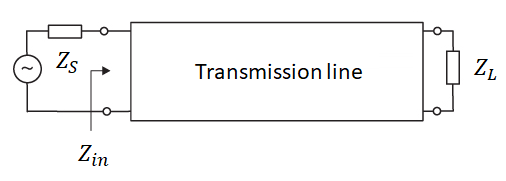
\includegraphics[width=0.5\textwidth]{figures/transmission_line.png}
            \caption{Transmission line schematic with input, source, and load impedances.}
        \end{figure}
        Hệ số phản xạ $\Gamma$\cite{cadence2023sparams}\cite{cadence2021transmission} biểu thị \textbf{mức độ sóng phản xạ lại} khi đi qua một giao diện có sự \textbf{không phù hợp trở kháng}\par
        
        \subsection{Hệ số phản xạ tại đầu tải}
            $$\Gamma_L = \frac{Z_{L} - Z_0}{Z_{L} + Z_0}$$
            \begin{itemize}
                \item $Z_{L}$: Trở kháng của tải (Load impedance)
                \item $Z_0$: Trở kháng đặc trưng của đường truyền
                \item $|\Gamma|$: Hệ số phản xạ, nằm trong khoảng $\left[0,1\right]$, giá trị càng lớn thì phản xạ càng cao
            \end{itemize}
        
        \subsection{Hệ số phản xạ tại nguồn}
            Phản xạ tại nguồn khi tín hiệu quay ngược về phía đầu vào của đường truyền:
            $$\Gamma_S = \frac{Z_{in} - Z_S}{Z_{in} + Z_S}$$
            \begin{itemize}
                \item $Z_{in}$: Trở kháng đầu vào của đường truyền
                \item $Z_S$: Trở kháng của nguồn
            \end{itemize}

    \section{Trở kháng đầu vào (Input Impedance)}
        Trở kháng đầu vào (Zin) là trở kháng mà nguồn nhìn thấy khi tín hiệu đi vào đường truyền.
        \begin{equation}
            Z_{in} = Z_0 \frac{Z_L + Z_0 \tanh(\gamma l)}{Z_0 + jZ_L \tanh(\gamma l)}
            \label{eq:zin}    
        \end{equation}
        
        \begin{itemize}
            \item $l$: Chiều dài đường truyền
        \end{itemize}

    \section{S11 (Return Loss)}
        Định nghĩa về return loss theo hệ số phản xạ đường truyền.
        $$RL = -10\log\left(\left|\frac{P_{ref}}{P_{inc}}\right|\right) = -20\log\left(\left|\frac{V_{ref}}{V_{inc}}\right|\right) = -20\log\left(\left|\Gamma\right|\right)$$
        Trở kháng đầu vào và S11 (return loss) đều liên quan đến hệ số phản xạ của đường truyền. Các tham số S thực là các hàm phức tạp của tần số và có thể có một tập hợp phức tạp các cộng hưởng/phản cộng hưởng (resonances/antiresonances); ví dụ về đường truyền được kết nối với điện dung tải 1 pF được kết thúc ở 50 Ohm được hiển thị bên dưới.\par
        \begin{figure}[h]
            \centering
            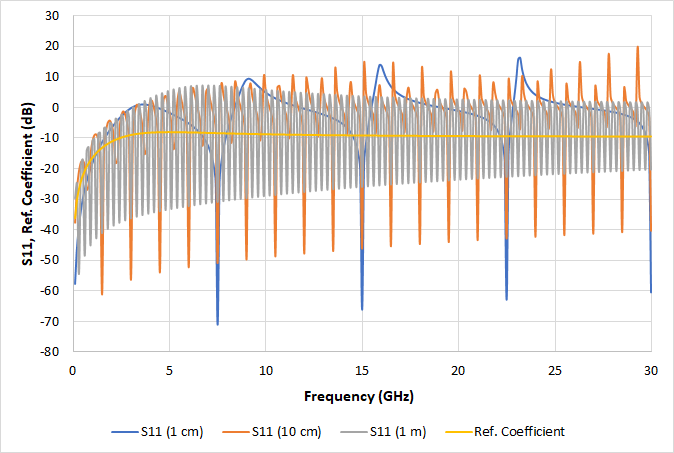
\includegraphics[width=0.5\textwidth]{figures/1pf_input.png}
            \caption{Comparison of S11 and reflection coefficient at the input to a load component with 1 pF input capacitance.}
        \end{figure}

        Đường truyền hoạt động giống như một khoang cộng hưởng điển hình\footnote{\href{https://resources.pcb.cadence.com/blog/2019-what-is-a-cavity-resonator-and-how-is-one-used-in-pcb-design}{\color{blue}What is a Cavity Resonator and How is One Used in PCB Design}} và có cấu trúc cộng hưởng khi đường truyền rất ngắn. khi đường truyền dài hơn, tổn thất bắt đầu chiếm ưu thế và cộng hưởng trong phổ S11 bắt đầu biến mất.\cite{cadence2021transmission}\par
        Khi kéo dài đường truyền ra vô cực, trở kháng đầu vào tại mỗi cổng giảm xuống (Phương trình \ref{eq:zin}). Đối với các đường truyền thực tế hoạt động ở tần số thực tế, cần phải mô tả hành vi tín hiệu theo trở kháng đầu vào và tham số S, đặc biệt là khi đường truyền ngắn.\cite{cadence2021transmission}\par